\section[Sequential CHC degradation with isotope fractionation (1D)]{1D reactive transport: Sequential CHC degradation with isotope fractionation}
\label{l_s_benchmark_isofrac}

\subsection{Reaction model}
When a substrate $C$ is present in the form of light and heavy isotopes $C^l$ and $C^h$ and one of the isotopes is preferentially consumed by a microbial population $X$, a kinetic isotope fractionation effect can be observed, i.e. one of the isotopes will become enriched in the remaining fraction of electron donors relative to its isotope partner. At the same time, the preferentially consumed isotope will become enriched in the reaction product relative to the more recalcitrant isotope. The degree of isotope fractionation can be expressed by means of the fractionation factor $\alpha$ [-], which is a reaction specific constant and relates the isotopic ratio of the degradation reaction's product to the isotope ratio of the substrate. Often, the the isotopic enrichment factor $\varepsilon $ [-] is used to quantify the isotope effect of a reaction, which can be related to $\alpha$ for a one step process by

\begin{equation}
    \varepsilon =  (\alpha -1)\cdot1000
    \label{iso_enrichfac}
\end{equation}

According to Van Breukelen et al.~\cite{VanBr:05}, the degradation rate of the light carbon isotope substrate $d^{12}C_S/dt$ is given by the overall degradation rate $dC_S/dt$ of substrate $C_S$ corrected for the proportion of $^{12}C_S$ to total $C_S$

\begin{equation}
    -\frac{d^{12}C_S}{dt} = \frac{d^{12}C_P}{dt} = -\frac{dC_S}{dt} \frac{^{12}C_S}{^{12}C_S + ^{13}C_S}
    \label{iso_rate_gen1}
\end{equation}

The degradation rate of the heavy isotope substrate $d^{13}C_S/dt$ then is given by

\begin{equation}
    -\frac{d^{13}C_S}{dt} = \frac{d^{13}C_P}{dt} = -\frac{dC_S}{dt} \frac{^{13}C_S}{^{12}C_S + ^{13}C_S}(\varepsilon\cdot10^{-3}+1)
    \label{iso_rate_gen2}
\end{equation}

$dC_S/dt$ can be any rate expression, such as first order, Michaelis-Menten or Monod-kinetics. Based on this concept and using the general formulation of multiple Monod kinetics of first order growth of a microbial species $X$ from consumption of the light isotope substrate $^{12}C_S$ can be expressed by

\begin{equation}
    \left[
    \frac{\partial X}{\partial t}
    \right]_{^{12}C_S}
    = \mu_{max} X\left[
    \prod_{j=1}^{n_M-1} \left( \frac{C_j}{K_{j}^M + C_j} \right)
    \prod_{j=1}^{n_I} \left( \frac{K_{j}^I}{K_{j}^I + C_j} \right)
    \right]
    \frac{C_S^{tot}}{C_S^{tot} + K_{C_S}^M}
    \frac{^{12}C_S}{C_S^{tot}}
    \label{iso_monod_light}
\end{equation}

where $C_S^{tot} = ^{12}C_S+^{13}C_S$ and $\mu_{max}$ [T$^{-1}$] is the maximum growth rate of $X$ with respect to substrate $C$. Growth of $X$ from consumption of the heavy isotope substrate $^{13}C_S$ can be expressed accordingly by


\begin{equation}
        \left[
    \frac{\partial X}{\partial t}
    \right]_{^{13}C_S}
    = \mu_{max}^{\ast} X\left[
    \prod_{j=1}^{n_M-1} \left( \frac{C_j}{K_{j}^M + C_j} \right)
    \prod_{j=1}^{n_I} \left( \frac{K_{j}^I}{K_{j}^I + C_j} \right)
    \right]
    \frac{C_S^{tot}}{C_S^{tot} + K_{C_S}^M}
    \frac{^{13}C_S}{C_S^{tot}}
    \label{iso_monod_heavy}
\end{equation}

where $\mu_{max}^{\ast}= \mu_{max}(\varepsilon/1000 -1)$. The resulting degradation rates of $^{12}C_S$ and $^{13}C_S$ accordingly are given by

\begin{equation}
    \frac{\partial ^{12}C_S}{\partial t} = -\mu_{max} X\frac{St_{C_S}}{Y_{C_S}}
    \left[
    \prod_{j=1}^{n_M-1} \left( \frac{C_j}{K_{j}^M + C_j} \right)
    \prod_{j=1}^{n_I} \left( \frac{K_{j}^I}{K_{j}^I + C_j} \right)
    \right]
    \frac{C_S^{tot}}{C_S^{tot} + K_{C_S}^M}
    \frac{^{12}C_S}{C_S^{tot}}
    \label{iso_monod_sub_light}
\end{equation}

\begin{equation}
    \frac{\partial ^{13}C_S}{\partial t} = -\mu_{max}^{\ast} X\frac{St_{C_S}}{Y_{C_S}}
    \left[
    \prod_{j=1}^{n_M-1} \left( \frac{C_j}{K_{j}^M + C_j} \right)
    \prod_{j=1}^{n_I} \left( \frac{K_{j}^I}{K_{j}^I + C_j} \right)
    \right]
    \frac{C_S^{tot}}{C_S^{tot} + K_{C_S}^M}
    \frac{^{13}C_S}{C_S^{tot}}
    \label{iso_monod_sub_heavy}
\end{equation}

where $St_{C_S}$ [-] and $Y_{C_S}$ [-] are the stoechiometric and yield coefficients for substrate $C_S$. Degradation kinetics for the conceptually more simple Michaelis-Menten, first or zeroth order kinetics may be derived on basis of eqs.~\ref{iso_monod_light} -~\ref{iso_monod_sub_heavy} assuming a constant microorganism mass and choosing appropriate values of $\mu_{max}$, $\mu_{max}^{\ast}$, $K^M_{C_S}$, $St_{C_S}$ and $Y_{C_S}$.

For the simulation of biodegradation with isotope fractionation of a substrate species $C_S$ by multiplicative Monod (or one of the more simplified) kinetics, heavy and light isotopes of the fractionating substrate, e.g.  $^{12}C_S$ and $^{13}C_S$, must be defined as two individual species with corresponding transport processes. Also, two individual degradation reactions must be defined, requiring identical parameter values for  $\mu_{max}$ , $Y_{C_S}$, and all $K^M_i$, $K^I_i$, and $St_i$. The isotopic enrichment factor $\varepsilon$ then is used to calculate the modified maximum growth rate $\mu_{max}^{\ast}$ for the more recalcitrant isotope.

\subsection{Definition}

In this benchmark, which is based on a model of ~\cite{VanBr:05}, sequential degradation of chlorinated hydrocarbons (CHC) from PCE to the end product ethylene (Eth), which is not further degraded, is simulated:

$PCE \rightarrow TCE \rightarrow DCE \rightarrow VC \rightarrow Eth $

A contaminant source located at the upstream model boundary emits a constant concentration of PCE. All degradation reactions follow simple first order kinetics and involve an isotope fractionation effect. The one-dimensional transport model has a length of 876 m and is discretized by 120 finite line elements of 7.3 m length, respectively. Basic flow and transport model parameters are summarized in Tab.~\ref{l_tab_benchmark_isofrac_flow}, reaction parameters for the individual species in Tab.~\ref{l_tab_benchmark_isofrac_react}.

\begin{table}[htbp]
\caption{Parameters used for benchmark}
\centering
\begin{tabular}{lrl}
\hline
Parameter & Value & Unit \\
\hline
porosity $\Phi = n $  & 0.25 &  --  \\			
matrix volume fraction $VOL\_MAT $  & 0.74 &  --  \\			
biomass volume fraction $VOL\_BIO $  & 0.01 &  --  \\			
hydraulic conductivity $K$ & 1.1574$\times 10^{-4}$ & $m \cdot s^{-1}$ \\
flow velocity $q$ & 1.1574$\times 10^{-6}$ & $m \cdot s^{-1}$ \\
longitudinal dispersivity $\alpha_l$ & 1.0 & $m$ \\
component diffusion coefficient $D$ & 3.0$\times 10^{-9}$ & $m \cdot s^{-1}$ \\
\hline
\end{tabular}
\label{l_tab_benchmark_isofrac_flow}
\end{table}


\begin{table}[htbp]
\caption{Reaction parameters used for benchmark HC$\backslash$1d\_isofrac }
\centering
\begin{tabular}{|l|l|l|}
\hline
CHC species & enrichment factor $\varepsilon$ [-] & first order rate constant $\lambda $ $[s^{-1}]$ \\
\hline
PCE & -5.2 & 6.366$\times 10^{-8}$ \\
\hline
TCE & -8.5 & 3.125$\times 10^{-8}$ \\
\hline
DCE &  -17.8 & 2.199$\times 10^{-8}$ \\
\hline
VC & -23.2 & 1.273$\times 10^{-8}$ \\
\hline
Eth & 0.0 & -- \\	
\hline
\end{tabular}
\label{l_tab_benchmark_isofrac_react}
\end{table}


Each of the mobile hydrocarbon species is defined twice, once for the light isotopologue and once for the respective heavy isotopologue. Also, an immobile microorganism species $X$ is defined, which has an initial unit concentration of 1.0 throughout the model domain. The microorganisms degrade each of the chlorinated species (i.e. PCE, TCE, DCE and VC). Thus, a total of eight monod-type growth reactions for $X$, one for each isotopologue species, must be defined. Growth of $X$, however, is inhibited by setting the growth parameter in the *.krc file to zero in each of the reactions and microorganism decay is not included in the simulation, i.e. $X$ is constant in time and space. Each reaction contains only a single Monod term for the respective isotopologue species. To achieve degradation kinetics of first order in each case, the half saturation concentrations $K^M_i >> C_i$ and are hence set to a value of 1.0$\times 10^{10}$. As the effective first order rate constant is given by $\lambda_i = \mu_{max_i} / K^M_i$, parameters $\mu_{max_i}$ are set to proportionally high values in the *.krc file, i.e. ten orders of magnitude larger than indicated in Tab.~\ref{l_tab_benchmark_isofrac_react}. Also, the yield coefficients $Y_i$ for the individual reactions must be set to 1.0.

Initial concentrations of all species except the microorganisms are 0.0 mol L$^{-1}$ throughout the model domain. For $^{12}$PCE and $^{13}$PCE the upgradient boundary conditions are constant concentrations of 9.892$\times$10$^{-4}$ and 1.078$\times$10$^{-4}$ mol L$^{-1}$, respectively. The hydraulic gradient of 0.01 is induced by fixed head boundary conditions of 10.0 and 9.781 m at the up- and downgradient model boundaries. The reactive transport simulation is run for a period of 20 a with 200 time steps of 3153600 s, respectively, and using an explicit-implicit time stepping scheme ($\theta$ = 0.5).

Model results are compared against the one-dimensional Domenico analytical solution including first order degradation kinetics as well as by comparison of an equivalent one dimensional simulation with PHREEQC, which was presented by Van Breukelen et al.~\cite{VanBr:05}. 

\subsection{Solution}

Results at the end of the simulation are presented in Figs.~\ref{profiles_isofrac_C_AS} and ~\ref{profiles_isofrac_C}.
In Fig.~\ref{profiles_isofrac_C_AS}, numerical simulation results for the PCE isotopologues in form of normalized concentrations C/C$_0$ are compared against results of the one-dimensional Domenico analytical solution including first order degradation, in which the first order degradation rate for the heavy PCE isotopologue $\lambda_{^{13}PCE} = \lambda_{^{12}PCE}(\varepsilon/1000 -1)$. Note that for the comparison with the analytical solution kinetic reactions are suppressed on the first node of the FE mesh (i.e. on the upstream model boundary in order to correctly represent the concentration boundary condition of the analytical solution. Concentrations of the PCE isotopologues match the analytical solution over a concentration range of more than 10 orders of magnitude. Also the resulting $\delta^{13}C$ [permil] isotope signatures, which were computed by

\begin{equation}
    \delta^{13} C =  \left(
    \frac{R_{C_i}}{R_{Ref}} -1
    \right)1000
    \label{isotop_signature}
\end{equation}

where $R_{C_i}$ [-] is the isotope ratio $^{13}{C_i}/^{12}{C_i}$ of species $C_i$ in the simulation, while $R_{Ref}$  [-] is the isotope ratio of the international standard, i.e. in this case the Vienna Pee Dee Belemnite (V-PDB; $R_{Ref}$ = 0.011237), match results of the analytical solution precisely, verifying the correctness of the  implementation.

\begin{figure}[htbp]
\centering
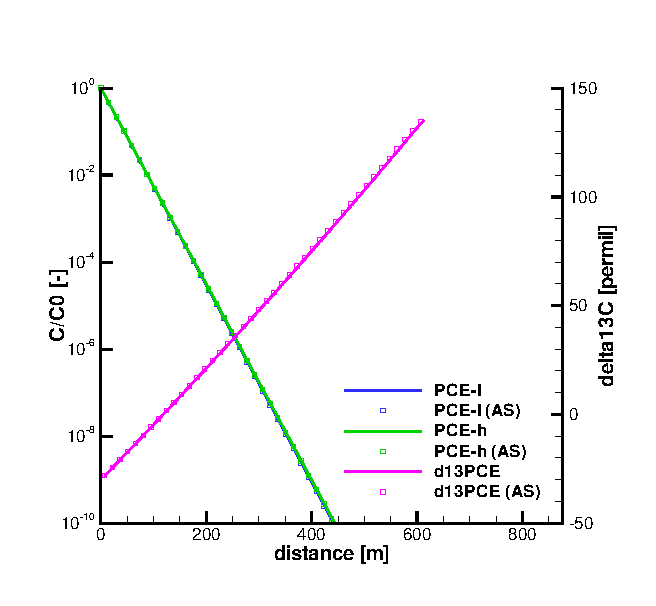
\includegraphics[width=0.6\textwidth]{PART_III/HC/Fig_isofrac_AS.eps}
\caption{PCE isotopologue concentration profiles (left axis) and $\delta^{13}C$ isotope signature (right axis) versus transport distance along the 1D model. Lines represent GeoSys simulation results, symbols represent analytical solution results.}
\label{profiles_isofrac_C_AS}
\end{figure}

\begin{figure}[htbp]
\centering
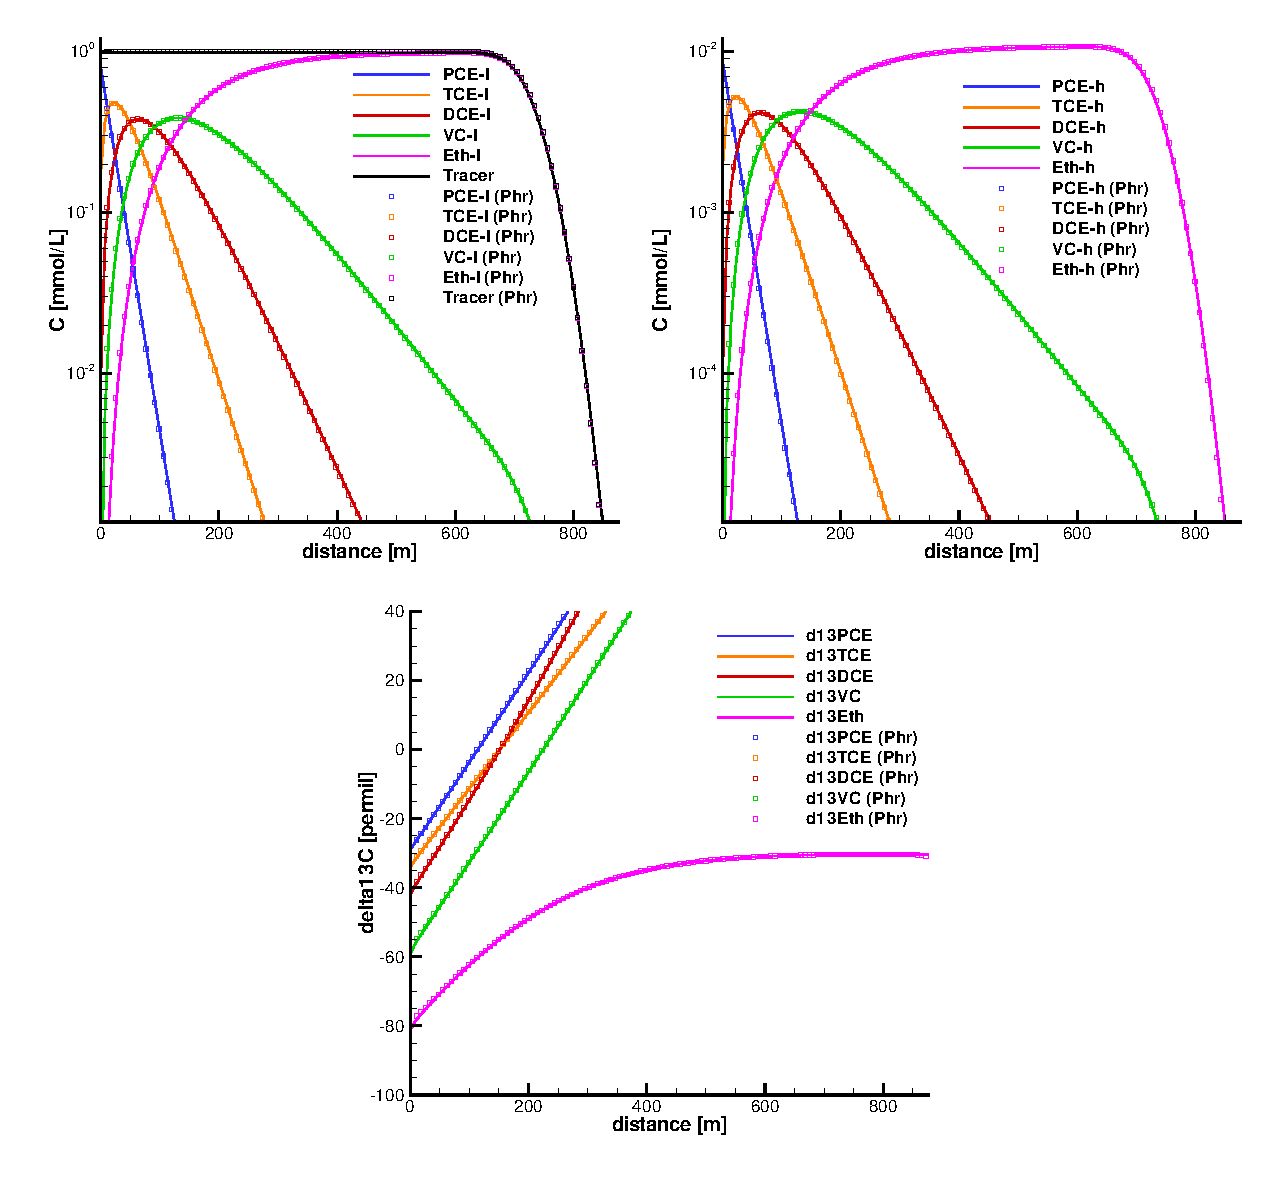
\includegraphics[width=1\textwidth]{PART_III/HC/Fig_isofrac_prof.eps}
\caption{Light (upper left diagram), heavy (upper right diagram) isotopologue chlorinated hydrocarbon species profiles and $\delta^{13}C$ isotope signatures (lower diagram) versus transport distance along the 1D model. Full lines represent GeoSys simulation results, symbols represent PHREEQC simulation results.}
\label{profiles_isofrac_C}
\end{figure}

In Fig.~\ref{profiles_isofrac_C} the upper left and right diagrams show simulated concentration profiles of the individual CHC species versus results obtained by PHREEQC. Note that for the comparison with the PHREEQC simulation, kinetic reactions are not suppressed on the upstream model boundary. The lower diagram shows $\delta^{13}C$ isotope signatures. While concentrations of $^{12}$PCE and $^{13}$PCE decrease exponentially with distance from the source at the left hand side model boundary, isotopologues of TCE, DCE and VC show concentration peaks in different distances from the source. Eth isotopologues finally accumulate as the end products of the degradation chain and reach the source concentrations of $^{12}$PCE and $^{13}$PCE, respectively. Also, while TCE, DCE and VC isotope signatures increase almost linearly with travel distance, demonstrating the increasing enrichment of the heavy isotopologues, the Eth signature approaches the $\delta^{13}C$ of the source, i.e. PCE. For all isotopologue species, concentration profiles and isotope signatures show an excellent agreement with the PHREEQC simulation, verifying the numerical implementation also for sequential degradation reactions.
